\documentclass[10pt]{beamer}

\usetheme{m}
\renewcommand{\mthemetitleformat}{\scshape\MakeLowercase}
\usepackage{booktabs}
\usepackage[scale=2]{ccicons}
\usepackage{cancel}
\usepgfplotslibrary{dateplot}
\usepackage{pdfpages}
\usepackage{graphicx}
\usepackage[export]{adjustbox}
\usepackage{enumitem}
\usepackage{fancyvrb}
\usepackage{verbatim}
\usepackage{setspace}
\usepackage{minted}
\usepackage[export]{adjustbox}

\newenvironment{abjadbookoutput}{}{}

\setmonofont[
    %BoldFeatures={FakeBold=3},
    %BoldFont=Inconsolata,
    %BoldItalicFeatures={FakeBold=3},
    %BoldItalicFont=Inconsolata,
    %ItalicFont=Inconsolata,
    Scale=MatchLowercase
]{Inconsolata}

\setminted{
    autogobble=true,
    fontsize=\footnotesize,
    frame=leftline,
    framerule=1.5pt,
    framesep=6pt,
    obeytabs=true,
    tabsize=4,
    xleftmargin=-6pt,
}

\newenvironment{markdown}{
    \VerbatimEnvironment
    \begin{VerbatimOut}{tmp/tmp.markdown}%
}{
    \end{VerbatimOut}
    \immediate\write18{pandoc tmp/tmp.markdown -t latex -o tmp/tmp.tex}
    \input{tmp/tmp.tex}
}

\setlist[description]{font=\normalfont\itshape}
\setlist[itemize]{font=\normalfont\itshape\textbullet\space}

\setlength{\arrayrulewidth}{0.2mm}
\setlength{\tabcolsep}{12pt}
\renewcommand{\arraystretch}{1.5}

\title{Constructing Musical Documents}
\subtitle{In Python With Abjad}
\author{
    Josiah Wolf Oberholtzer %\inst{1} \and
}
%\institute[shortinst]{
%    \inst{1}Department of Music, Harvard University
%}
\date[]{
    PDX Python\protect\\
    (Thursday 22 October 2015)
}

\begin{document}

\maketitle

\begin{frame}{Follow along}
\begin{block}{Project repository}
https://github.com/Abjad/abjad
\end{block}
\begin{block}{Presentation repository}
https://github.com/Abjad/presentations/tree/master/pdxpython
\end{block}
\begin{block}{Project documentation}
http://abjad.mbrsi.org
\end{block}
\end{frame}

\begin{frame}[fragile]{Who am I?}
\begin{markdown}
- Classically-trained composer
    - Acoustic chamber music 
    - Multi-channel electro-acoustic music
- Harvard, M.A., PhD, music composition
- MIT Music and Theater Arts
    - programmer for the Music21 project
- Forced Exposure (music distributor)
- Oberlin Conservatory, BMus, music composition
- I love Python
\end{markdown}
\end{frame}

\begin{frame}[fragile]{Abjad}
\begin{markdown}
The **Abjad API for Formalized Score Control** extends the Python
programming language with an open-source, object-oriented model of
common-practice music notation that enables composers to build scores
through the aggregation of elemental notation objects.
\end{markdown}
\end{frame}

\begin{frame}[fragile]{Dramatis Personae}
\begin{block}{Python}Needs no introduction.\end{block}
\begin{block}{LaTeX}A venerable automated typesetter.\end{block}
\begin{block}{LilyPond}LaTeX-inspired automated music engraving.\end{block}
\begin{block}{Graphviz}Automated graph / network visualization.\end{block}
\begin{block}{Abjad}A lot of glue.\end{block}
\end{frame}

\begin{frame}
    \frametitle{Table of Contents}
    \setbeamertemplate{section in toc}[sections numbered]
    \tableofcontents[hideallsubsections]
\end{frame}

\section{A little history}

\begin{frame}{}
\vfill
\begin{centering}
\textit{Music is poetry.\\ It's also math.\\ A lot of math.\\}
\end{centering}
\vfill
\end{frame}

\begin{frame}{Harmonic ratios}
    \begin{figure}
    \begin{centering}
    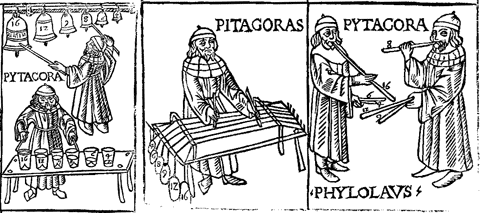
\includegraphics[max width=\textwidth]{assets/include-pythagoras.png}
    \caption{\emph{Pyth(on)agoras}: integer ratios dictating harmony}
    \end{centering}
    \end{figure}
\end{frame}

\begin{frame}{Rule-based music: constraints}
    \begin{figure}
    \begin{centering}
    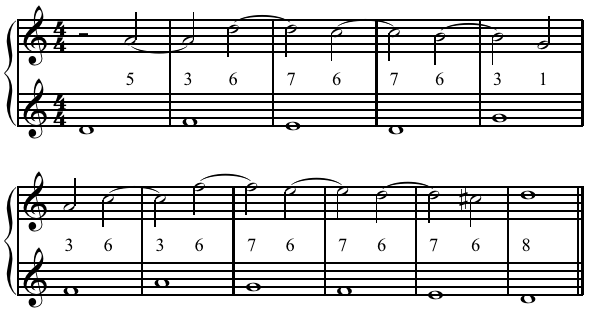
\includegraphics[height=2.25in]{assets/include-species-counterpoint.png}
    \caption{\emph{Species counterpoint}: a constraint-satisfaction-problem dream}
    \end{centering}
    \end{figure}
\end{frame}

\begin{frame}{Random music}
    \begin{figure}
    \begin{centering}
    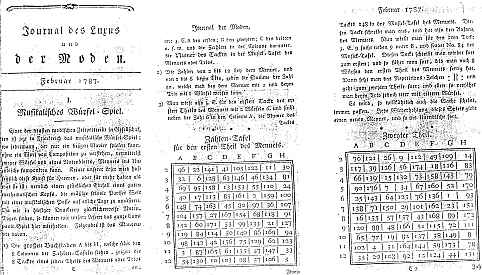
\includegraphics[height=2.25in]{assets/include-dice-game.jpg}
    \caption{Random minuets via Mozart's Dice Game}
    \end{centering}
    \end{figure}
\end{frame}

\begin{frame}{Xenakis}
    \begin{figure}
    \begin{centering}
    \begin{tabular}{cc}
    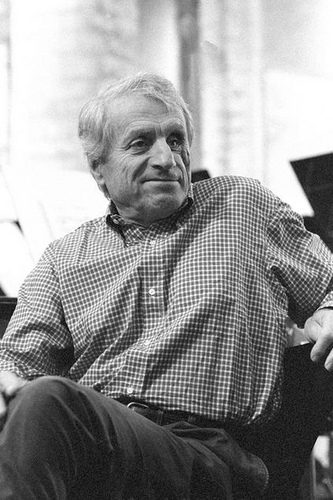
\includegraphics[height=2.25in]{assets/include-xenakis-portrait.jpg}
    &
    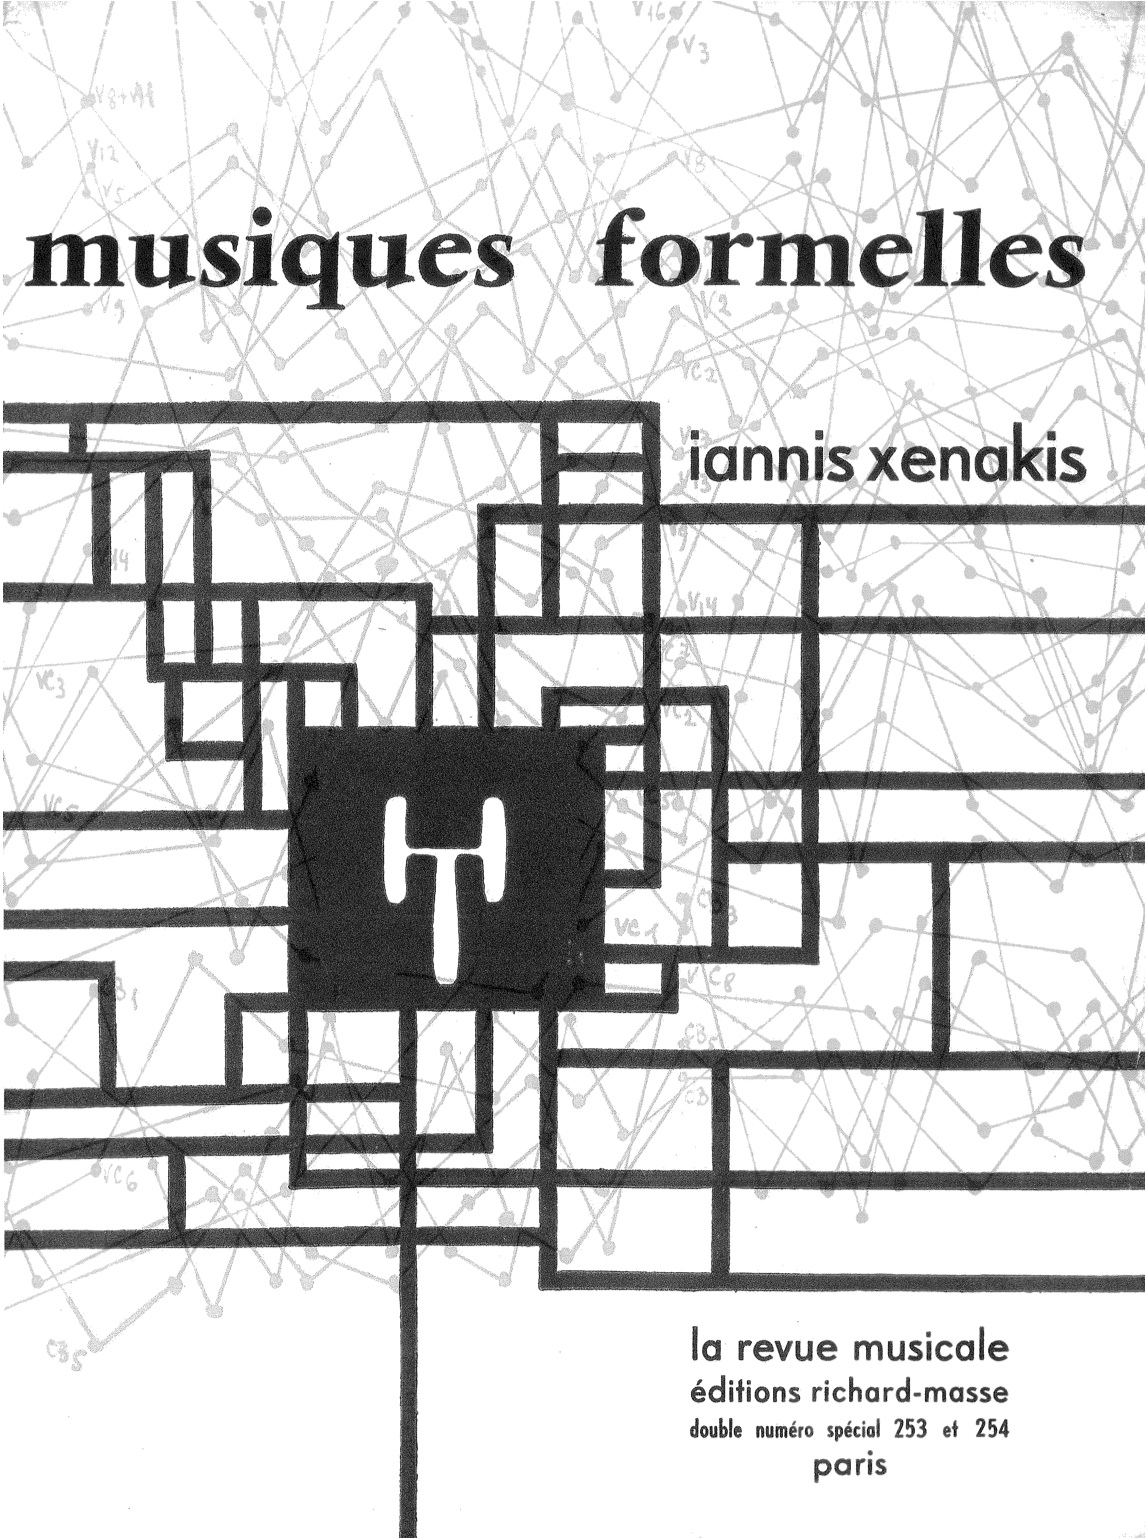
\includegraphics[height=2.25in]{assets/include-xenakis-formalized-music.jpg}
    \end{tabular}
    \caption{Iannis Xenakis (1922-2001)}
    \end{centering}
    \end{figure}
\end{frame}

\begin{frame}{Stochasticism}
    \begin{figure}
    \begin{centering}
    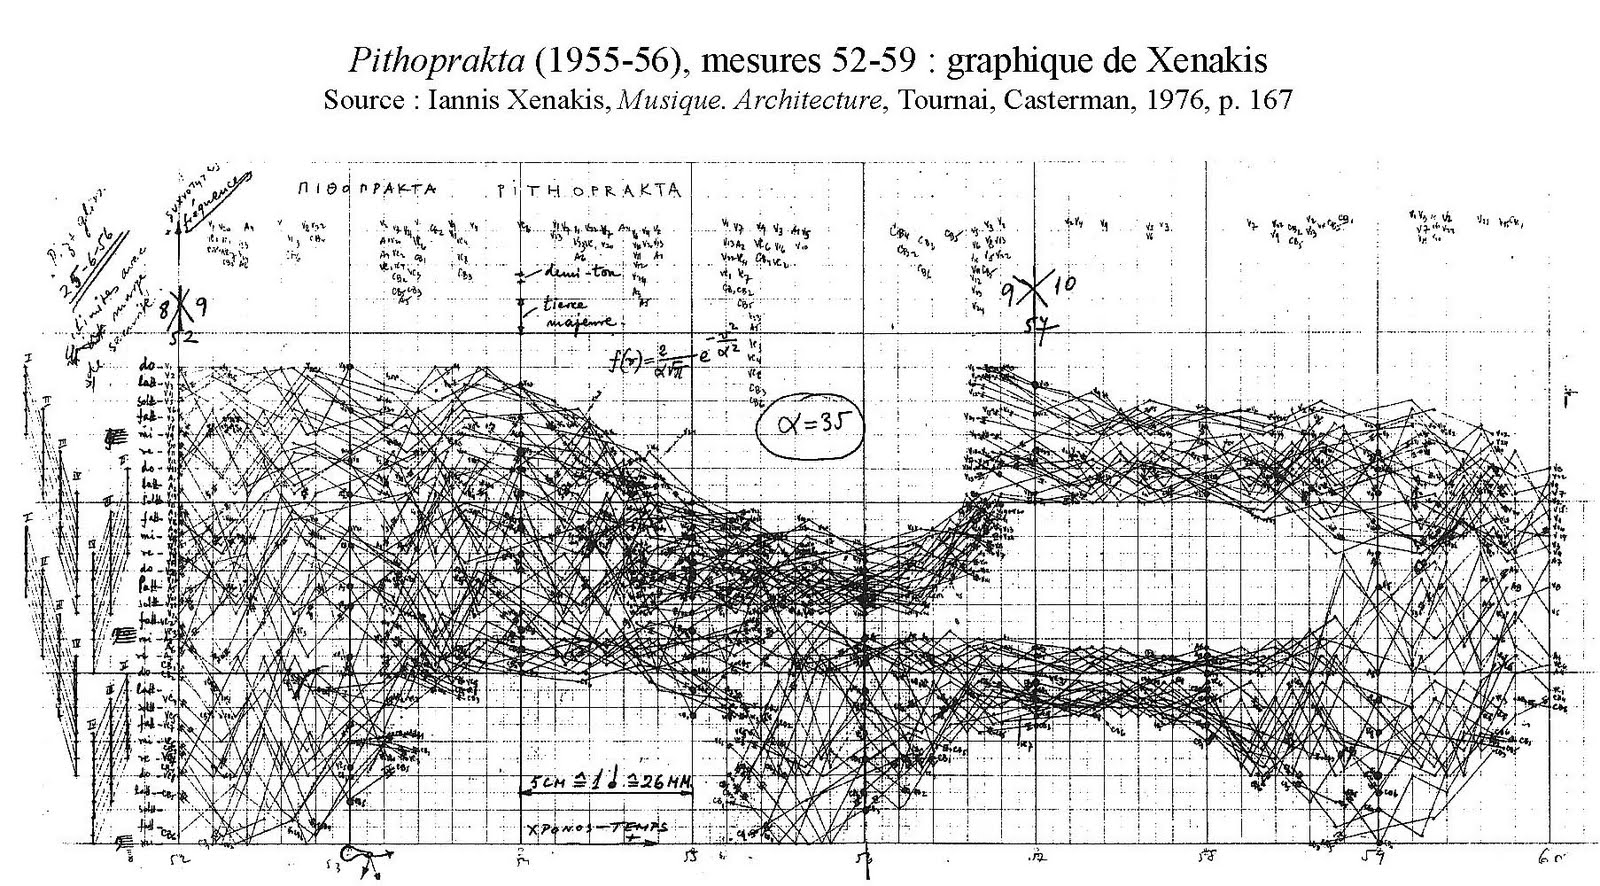
\includegraphics[max width=\linewidth]{assets/include-xenakis-pithoprakta.jpg}
    \caption{Stochastic string orchestra trajectories}
    \end{centering}
    \end{figure}
\end{frame}

\begin{frame}{Spectral analysis}
    \begin{figure}
    \begin{centering}
    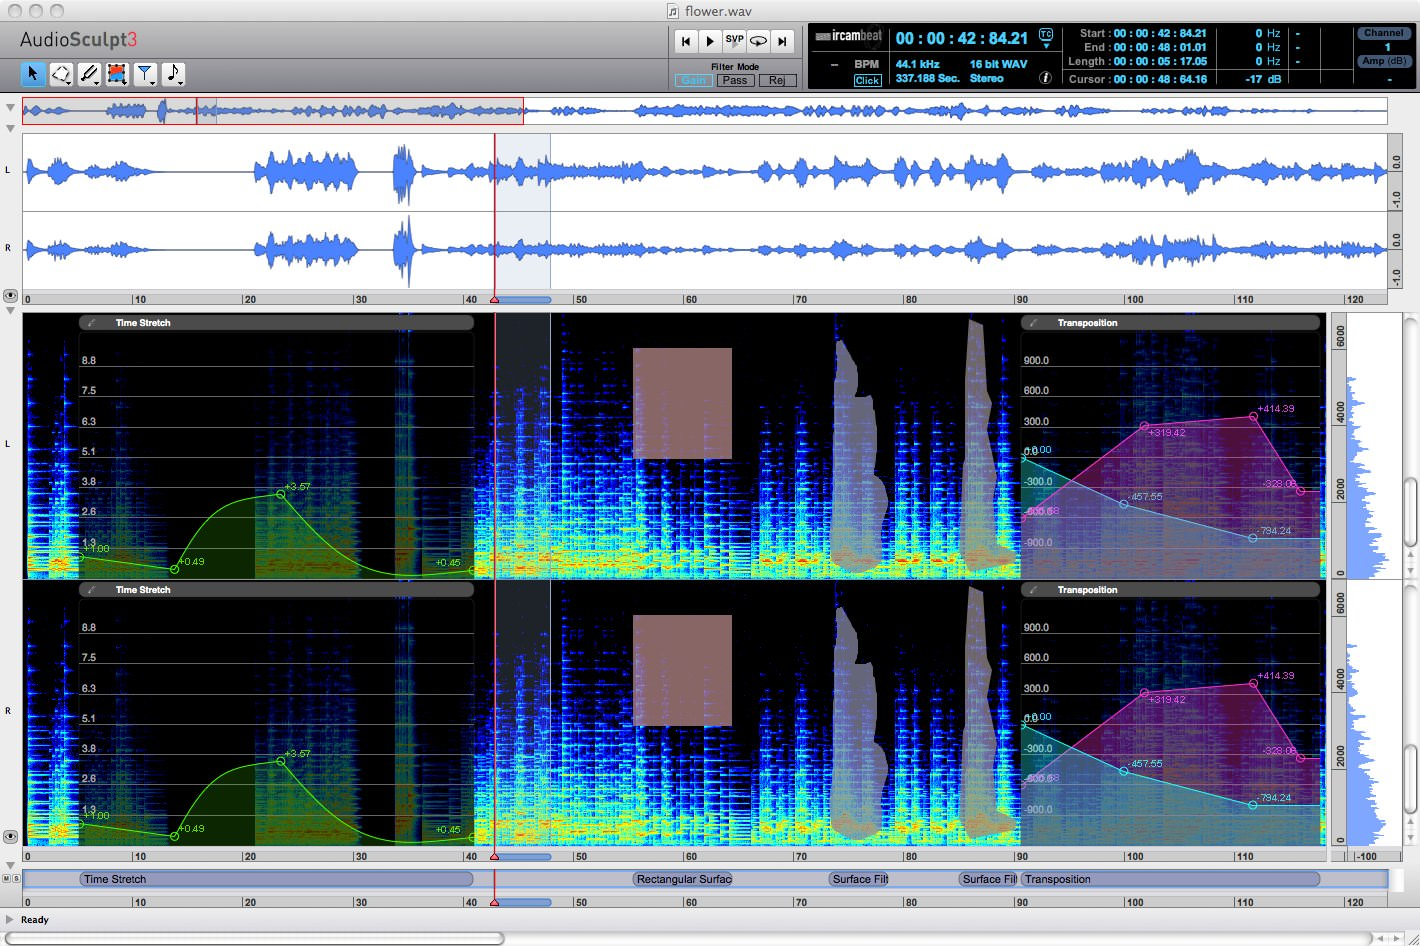
\includegraphics[height=2in]{assets/include-audiosculpt.jpg}
    \caption{IRCAM's AudioSculpt}
    \end{centering}
    \end{figure}
\end{frame}

\begin{frame}{Lisp, lots of Lisp, fields of Lisp, a tremendous amount of Lisp}
    \begin{figure}
    \begin{centering}
    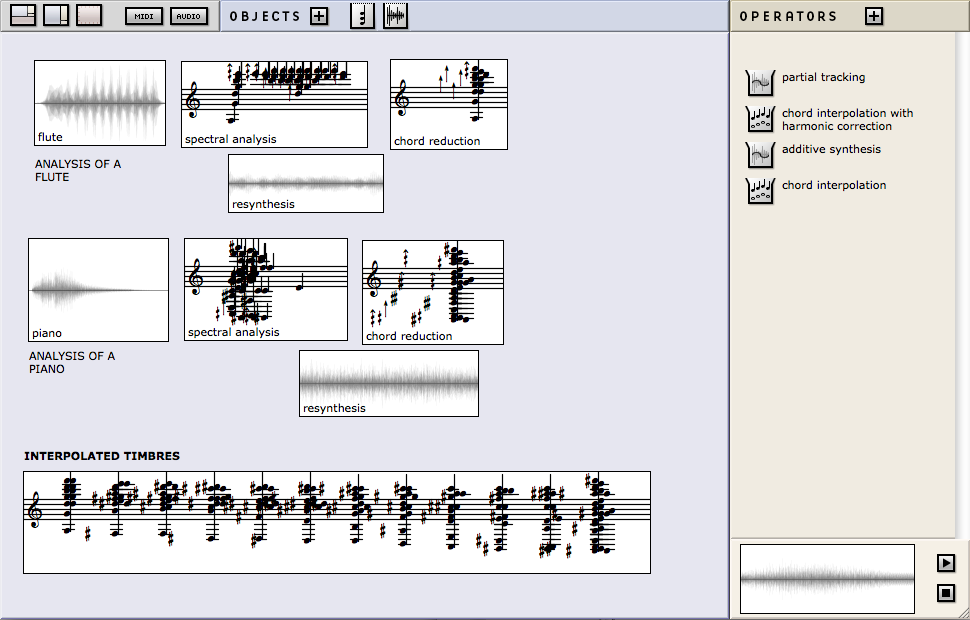
\includegraphics[height=2in]{assets/include-open-music.png}
    \caption{OpenMusic: Lisp hidden behind boxes}
    \end{centering}
    \end{figure}
\end{frame}

\begin{frame}{Yellow Lisp, red Lisp, Lisp with feathers, cream of Lisp}
    \begin{figure}
    \begin{centering}
    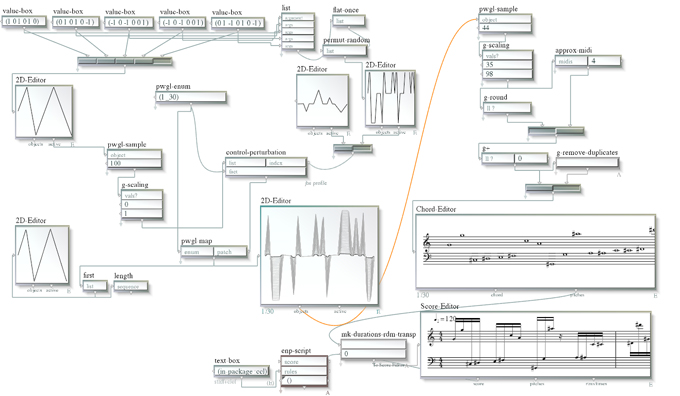
\includegraphics[height=2in]{assets/include-pwgl.jpg}
    \caption{PWGL: yet more Lisp hidden behind boxes}
    \end{centering}
    \end{figure}
\end{frame}

\begin{frame}{Boxes and Lines}
    \begin{figure}
    \begin{centering}
    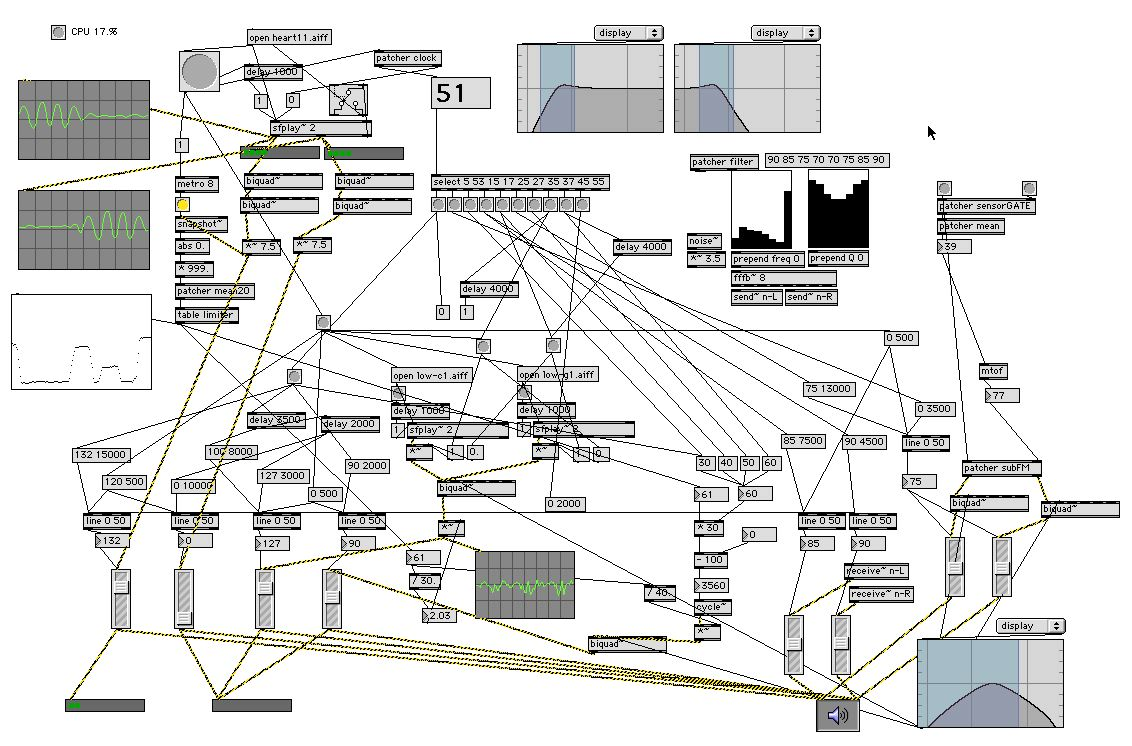
\includegraphics[height=2.25in]{assets/include-max.jpg}
    \caption{Max/MSP: spaghetti code as cautionary tale or design goal?}
    \end{centering}
    \end{figure}
\end{frame}
\begin{frame}[fragile]{Abjad history}
\begin{markdown}
- C into Finale via MIDI (1997)
- Mathematica into Sibelius via MIDI (2001)
- Mathematica into SCORE (2003)
- Mathematica into LilyPond (2004)
- Python into Adobe Illustrator (2004)
- Python into LilyPond (2005)
- Max/MSP into MS Access into Adobe Illustrator (2008)
- Public release on GoogleCode (2008)
- Migration to GitHub (2011)
- Abjad 2.16 released (2015)
\end{markdown}
\end{frame}

\begin{frame}[fragile]{Problems}
\begin{markdown}
We want:

- Ease of use
- Extensibility
- Stability
- Publication-quality typesetting
- To just make some music

We don't want:

- To learn how PostScript works
- To juggle Bezier curve control points
- To even think about kerning
- To reinvent the wheel, no matter how much fun
\end{markdown}
\end{frame}

\begin{frame}{Stack}
\begin{table}
    \caption{Abjad's Software Stack}
    \begin{tabular}{ |c|c|c|c|c| }
        \hline
        \multicolumn{5}{|c|}{\textbf{Python}} \\
        \hline
        \multicolumn{5}{|c|}{\textbf{Abjad}} \\
        \hline
        \xcancel{\textbf{SCORE}} & \textbf{LilyPond} & \textbf{Steinberg?} & ... & ... \\
        \hline
    \end{tabular}
\end{table}
\end{frame}

\begin{frame}[fragile]{LaTeX, LilyPond \& Graphviz}
\begin{markdown}
- Automated typesetting systems
- What-You-See-Is-What-You-Mean
- Available on the command-line
- Extensible / modular / allow scripting
- Take plain-text as input
- Give back beautiful graphics as output
- Oh, and Python isn't half-bad at...
    - Writing out plain text files, and...
    - Opening shells to command-line programs
\end{markdown}
\end{frame}
\section{Live coding}
\section{Abjad's object model}

\begin{frame}{Object model}
    \begin{block}
        {Abjad models musical score as a tree of components}
        Containers, leaves, spanners \& indicators
    \end{block}
    \begin{block}
        {Relationships between objects are modeled explicitly}
        Parentage, lineage, logical tie, logical voice
    \end{block}
    \begin{block}
        {Primitive objects are also modeled explicitly}
        Duration, Offset, Pitch, PitchClass, Interval, Octave, Accidental
    \end{block}
    \begin{block}
        {Top-level functions expose higher-level interfaces}
        Inspection, iteration, selection, mutation, persistence
    \end{block}
\end{frame}

\begin{frame}{Containers, leaves \& spanners}
    \begin{figure}
    \begin{centering}
        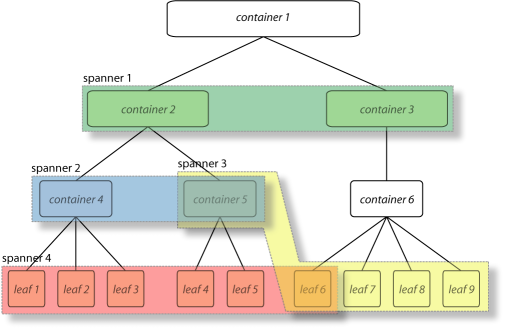
\includegraphics[height=2.5in]{assets/include-container-spanner.png}
    \caption{Spanners introducing cyclicity}
    \end{centering}
    \end{figure}
\end{frame}

\begin{frame}[fragile]{Parsers}
\begin{markdown}
- PLY-powered
- Pervasive throughout the system
- LilyPond syntax parsing
    - Includes a Scheme parser for LilyPond's embedded Scheme-Lisp
- IRCAM-inspired RTM-parsing
- *Reduced-LilyPond*-parsing for pedagogical examples
\end{markdown}
\end{frame}

\begin{frame}[fragile]{A two voice example}
\begin{comment}
<abjad>
upper_staff_string = "abj: | 5/8 c'8 r8 d'4 e'8 || 7/8 e'8 r8 fs'2 g'8 |"
lower_staff_string = "abj: | 5/8 c4. b8 r8 || 7/8 3/4 { c8 a8 af8 bf8 } c'4 b4 |"
upper_staff= Staff(upper_staff_string, name='Upper Staff')
lower_staff = Staff(lower_staff_string, name='Lower Staff')
staff_group = StaffGroup(name='Staff Group')
staff_group.extend([upper_staff, lower_staff])
score = Score(name='Score')
score.append(staff_group)
show(score)
</abjad>
\end{comment}

\begin{abjadbookoutput}
\begin{singlespacing}
\vspace{-0.5\baselineskip}
\begin{minted}{pycon}
>>> upper_staff_string = "abj: | 5/8 c'8 r8 d'4 e'8 || 7/8 e'8 r8 fs'2 g'8 |"
>>> lower_staff_string = "abj: | 5/8 c4. b8 r8 || 7/8 3/4 { c8 a8 af8 bf8 } c'4 b4 |"
>>> upper_staff= Staff(upper_staff_string, name='Upper Staff')
>>> lower_staff = Staff(lower_staff_string, name='Lower Staff')
>>> staff_group = StaffGroup(name='Staff Group')
>>> staff_group.extend([upper_staff, lower_staff])
>>> score = Score(name='Score')
>>> score.append(staff_group)
>>> show(score)
\end{minted}
\noindent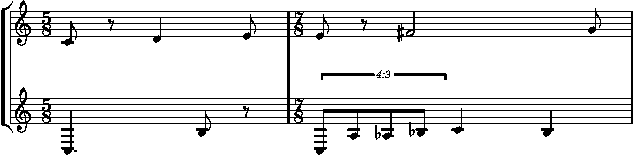
\includegraphics[max width=\textwidth,]{assets/lilypond-e3b1c40a4191d3949ecaa427d7f31b59.pdf}
\end{singlespacing}
\end{abjadbookoutput}

\end{frame}

\begin{frame}[fragile]{Top-level functions}
    \begin{block}{show(), play() and graph()}
        \emph{Illustratable} visualization or sonification
    \end{block}
    \begin{block}{attach(), detach()}
        Indicator and spanner attachment
    \end{block}
    \begin{block}{inspect\_()}
        Reveals inspection interface,\\
        Accesses score-context-derived info\\
        (How much work should properties do?)
    \end{block}
    \begin{block}{iterate()}
        Reveals interation interface
    \end{block}
\end{frame}

\begin{frame}[fragile]{Top-level functions}
    \begin{block}{mutate()}
        Reveals mutation interface
    \end{block}
    \begin{block}{override(), set\_()}
        Override and set LilyPond typographic overrides
    \end{block}
    \begin{block}{persist()}
        Reveals persistence interface,\\
        Exports objects as PNG, PDF, LilyPond, MIDI, etc.
    \end{block}
    \begin{block}{new()}
        \emph{Storage-formattable} object templating
    \end{block}
\end{frame}

\begin{frame}[fragile]{Showing, playing, graphing components}
\begin{comment}
<abjad>
show(score)
</abjad>
\end{comment}

\begin{abjadbookoutput}
\begin{singlespacing}
\vspace{-0.5\baselineskip}
\begin{minted}{pycon}
>>> show(score)
\end{minted}
\noindent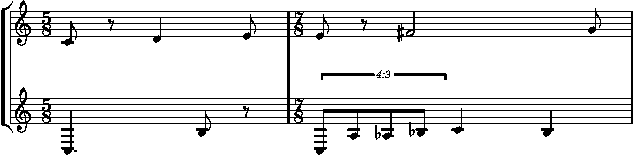
\includegraphics[max width=\textwidth,]{assets/lilypond-e3b1c40a4191d3949ecaa427d7f31b59.pdf}
\end{singlespacing}
\end{abjadbookoutput}

\end{frame}

\begin{frame}[fragile]{Showing, playing, graphing components}
\begin{comment}
<abjad>
graph(score)
</abjad>
\end{comment}

\begin{abjadbookoutput}
\begin{singlespacing}
\vspace{-0.5\baselineskip}
\begin{minted}{pycon}
>>> graph(score)
\end{minted}
\noindent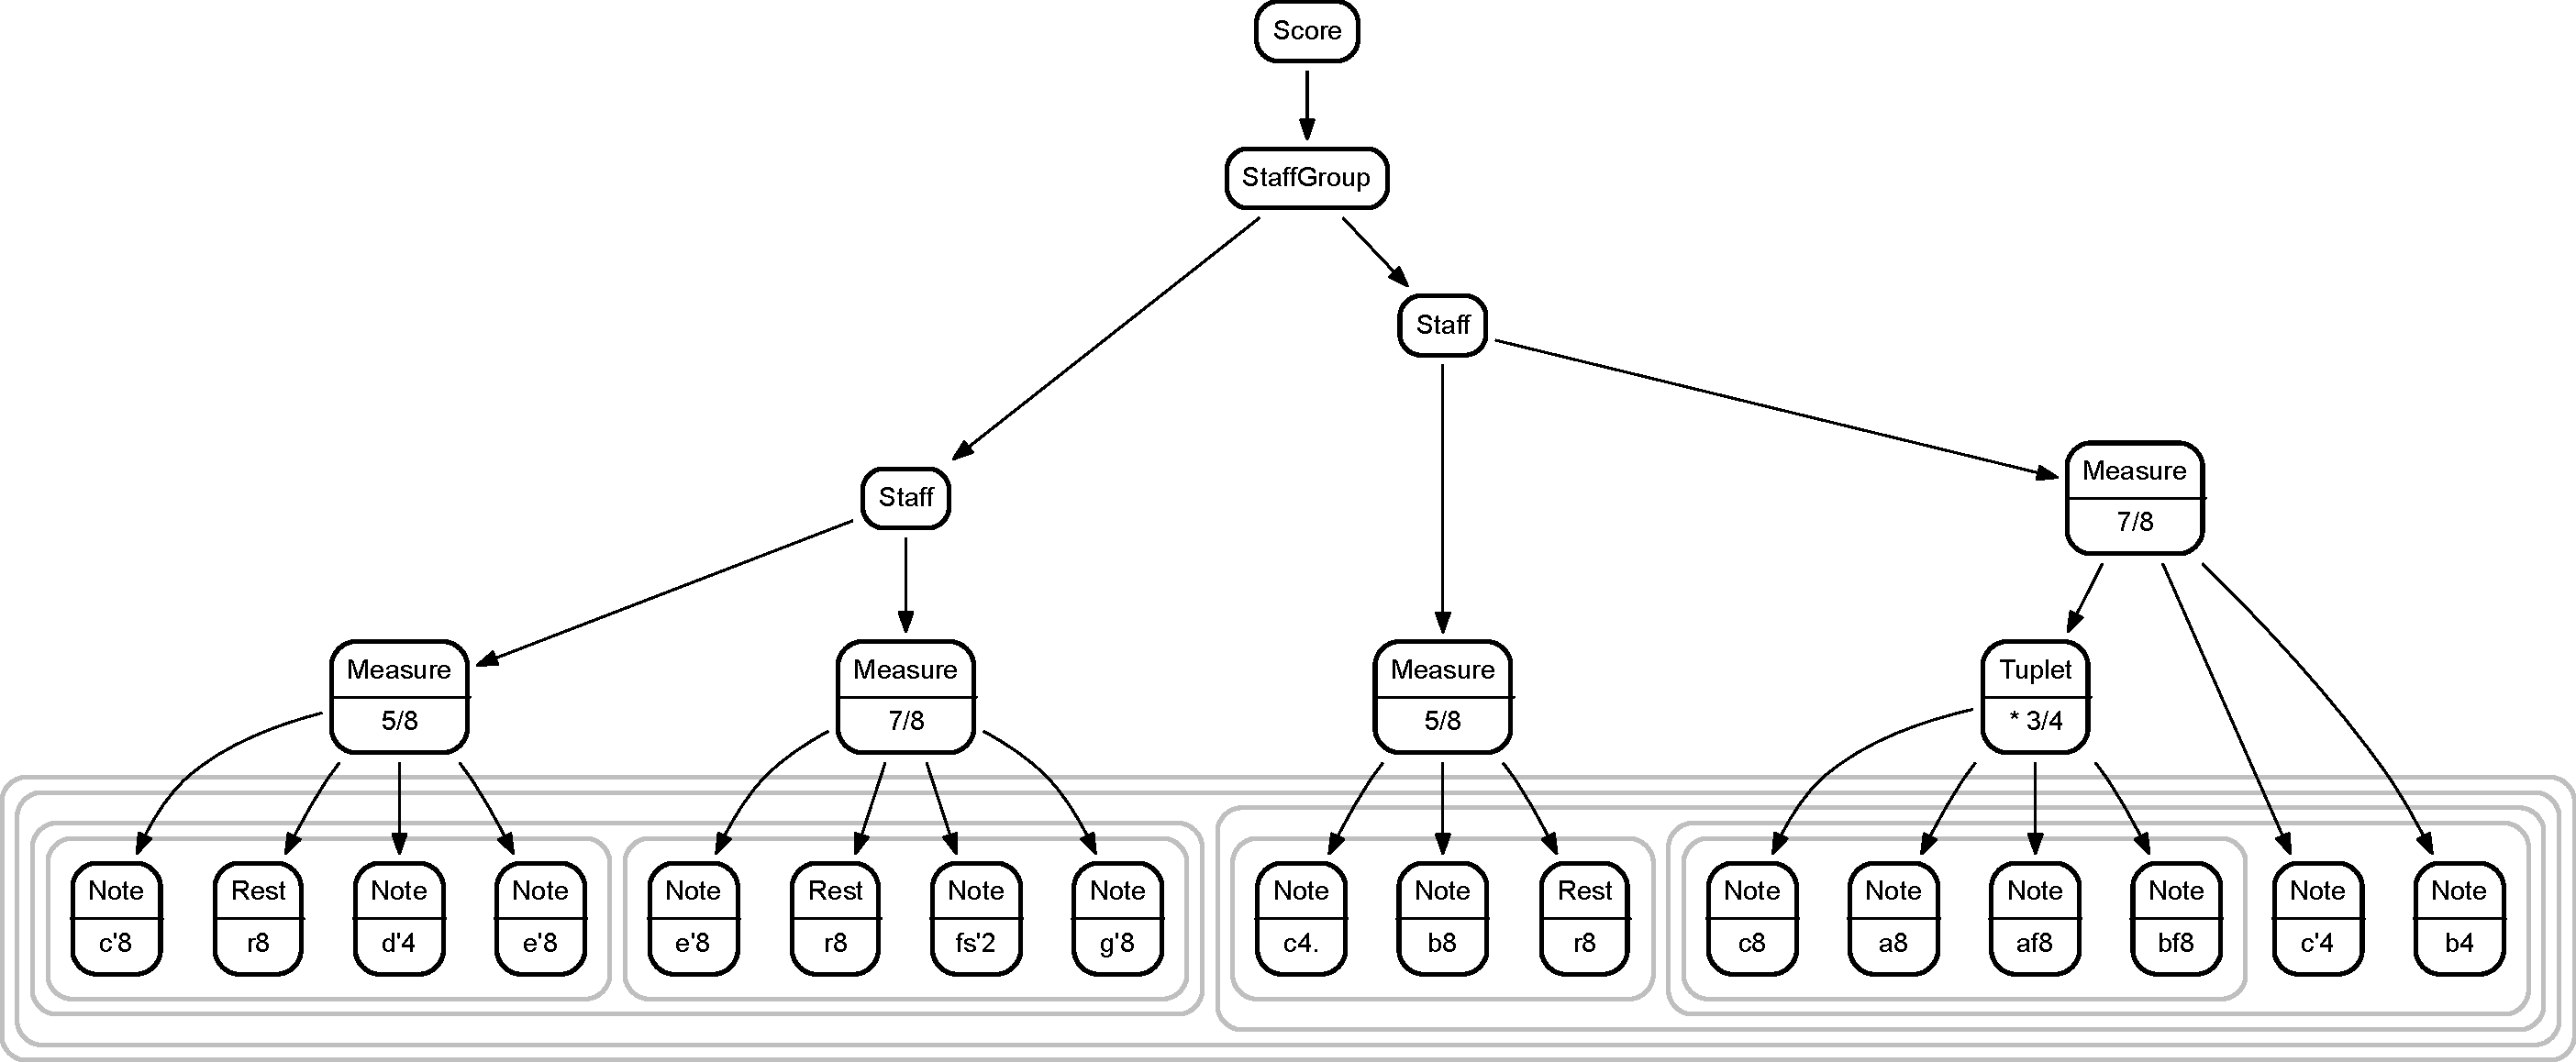
\includegraphics[scale=0.4,max width=\textwidth,]{assets/graphviz-e2c3abddd31202013f11968c9bff5808.pdf}
\end{singlespacing}
\end{abjadbookoutput}

\end{frame}

\begin{frame}[fragile]{Attaching and detaching}
\begin{comment}
<abjad>
attach(Tempo((1, 4), 56), upper_staff[0][0])
attach(Hairpin('p < f'), upper_staff[:])
to_tie_together = (upper_staff[0][-1], upper_staff[1][0])
attach(Tie(), to_tie_together)
show(score)
</abjad>
\end{comment}

\begin{abjadbookoutput}
\begin{singlespacing}
\vspace{-0.5\baselineskip}
\begin{minted}{pycon}
>>> attach(Tempo((1, 4), 56), upper_staff[0][0])
>>> attach(Hairpin('p < f'), upper_staff[:])
>>> to_tie_together = (upper_staff[0][-1], upper_staff[1][0])
>>> attach(Tie(), to_tie_together)
>>> show(score)
\end{minted}
\noindent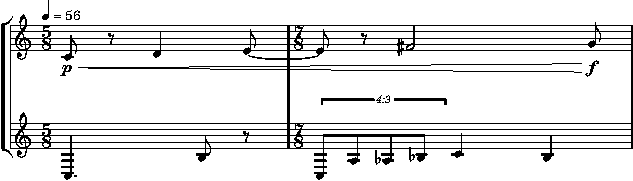
\includegraphics[max width=\textwidth,]{assets/lilypond-93a2b38978bbd78fc9e299d85430127a.pdf}
\end{singlespacing}
\end{abjadbookoutput}

\end{frame}

\begin{frame}[fragile]{Inspecting components}
\begin{comment}
<abjad>
inspect_(score).get_duration()
for component in inspect_(upper_staff[0]).get_parentage():
    component

inspect_(lower_staff[1]).get_timespan()
</abjad>
\end{comment}

\begin{abjadbookoutput}
\begin{singlespacing}
\vspace{-0.5\baselineskip}
\begin{minted}{pycon}
>>> inspect_(score).get_duration()
Duration(3, 2)
\end{minted}
\begin{minted}{pycon}
>>> for component in inspect_(upper_staff[0]).get_parentage():
...     component
...
Measure((5, 8), "c'8 r8 d'4 e'8 ~")
<Staff-"Upper Staff"{2}>
<StaffGroup-"Staff Group"<<2>>>
<Score-"Score"<<1>>>
\end{minted}
\begin{minted}{pycon}
>>> inspect_(lower_staff[1]).get_timespan()
Timespan(start_offset=Offset(5, 8), stop_offset=Offset(3, 2))
\end{minted}
\end{singlespacing}
\end{abjadbookoutput}

\end{frame}

\begin{frame}[fragile]{Indicator Scope}
\begin{markdown}
- Arbitrary objects can be attached to components
- They can be attached with *scope*
- Scoped objects *persist* until replaced
- Indicator scope can apply at different context levels
\end{markdown}
\begin{comment}
<abjad>
inspect_(score[0][1][1][-1]).get_effective(Tempo)
</abjad>
\end{comment}

\begin{abjadbookoutput}
\begin{singlespacing}
\vspace{-0.5\baselineskip}
\begin{minted}{pycon}
>>> inspect_(score[0][1][1][-1]).get_effective(Tempo)
Tempo(reference_duration=Duration(1, 4), units_per_minute=56)
\end{minted}
\end{singlespacing}
\end{abjadbookoutput}

\end{frame}

\begin{frame}[fragile]{Named components, Selecting leaves}
\begin{comment}
<abjad>
lower_staff = score['Lower Staff']
show(lower_staff)
lower_leaves = lower_staff.select_leaves()
inspect_(lower_leaves[-1]).get_effective(Tempo)
</abjad>
\end{comment}

\begin{abjadbookoutput}
\begin{singlespacing}
\vspace{-0.5\baselineskip}
\begin{minted}{pycon}
>>> lower_staff = score['Lower Staff']
>>> show(lower_staff)
\end{minted}
\noindent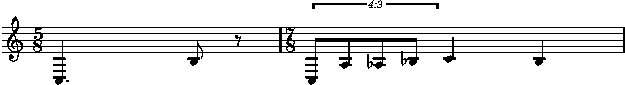
\includegraphics[max width=\textwidth,]{assets/lilypond-186cde23c908e6e806ba5e607f61aec2.pdf}
\begin{minted}{pycon}
>>> lower_leaves = lower_staff.select_leaves()
>>> inspect_(lower_leaves[-1]).get_effective(Tempo)
Tempo(reference_duration=Duration(1, 4), units_per_minute=56)
\end{minted}
\end{singlespacing}
\end{abjadbookoutput}

\end{frame}

\begin{frame}[fragile]{Iterating components}
\begin{comment}
<abjad>
iterator = iterate(score).depth_first()
for i, component in enumerate(iterator):
    print(component)
    if 6 < i:
        break

</abjad>
\end{comment}

\begin{abjadbookoutput}
\begin{singlespacing}
\vspace{-0.5\baselineskip}
\begin{minted}{pycon}
>>> iterator = iterate(score).depth_first()
>>> for i, component in enumerate(iterator):
...     print(component)
...     if 6 < i:
...         break
...
<Score-"Score"<<1>>>
<StaffGroup-"Staff Group"<<2>>>
<Staff-"Upper Staff"{2}>
Measure((5, 8), "c'8 r8 d'4 e'8 ~")
c'8
r8
d'4
e'8
\end{minted}
\end{singlespacing}
\end{abjadbookoutput}

\end{frame}

\begin{frame}[fragile]{Iterating components}
\begin{comment}
<abjad>
iterator = iterate(score).by_timeline_and_logical_tie()
for index, logical_tie in enumerate(iterator):
    attach(Markup(index).circle(), logical_tie.head)

show(score)
</abjad>
\end{comment}

\begin{abjadbookoutput}
\begin{singlespacing}
\vspace{-0.5\baselineskip}
\begin{minted}{pycon}
>>> iterator = iterate(score).by_timeline_and_logical_tie()
>>> for index, logical_tie in enumerate(iterator):
...     attach(Markup(index).circle(), logical_tie.head)
...
>>> show(score)
\end{minted}
\noindent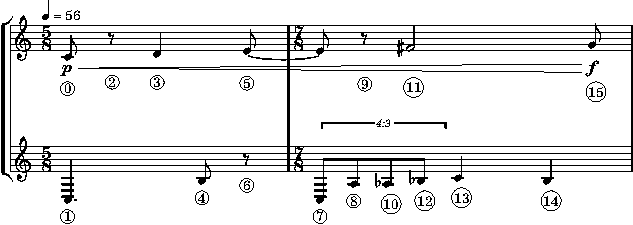
\includegraphics[max width=\textwidth,]{assets/lilypond-e9e234b6cc72814df926851d4e073617.pdf}
\end{singlespacing}
\end{abjadbookoutput}

\end{frame}

\begin{frame}[fragile]{Iterating components}
\begin{comment}
<abjad>
for leaf in iterate(score).by_class(scoretools.Leaf):
    detached_markup = detach(Markup, leaf)

show(score)
</abjad>
\end{comment}

\begin{abjadbookoutput}
\begin{singlespacing}
\vspace{-0.5\baselineskip}
\begin{minted}{pycon}
>>> for leaf in iterate(score).by_class(scoretools.Leaf):
...     detached_markup = detach(Markup, leaf)
...
>>> show(score)
\end{minted}
\noindent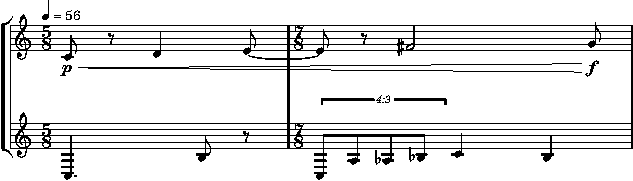
\includegraphics[max width=\textwidth,]{assets/lilypond-93a2b38978bbd78fc9e299d85430127a.pdf}
\end{singlespacing}
\end{abjadbookoutput}

\end{frame}

\begin{frame}[fragile]{Markup}
\end{frame}

\begin{frame}[fragile]{Generative component selectors}
\begin{comment}
<abjad>
selector = selectortools.Selector().by_leaves().by_run((Note, Chord))
for selection in selector.by_length('>', 1)(upper_staff):
    attach(Slur(), selection)

for leaf in selector[0].flatten()(upper_staff):
    attach(Articulation('accent'), leaf)

show(upper_staff)
</abjad>
\end{comment}

\begin{abjadbookoutput}
\begin{singlespacing}
\vspace{-0.5\baselineskip}
\begin{minted}{pycon}
>>> selector = selectortools.Selector().by_leaves().by_run((Note, Chord))
>>> for selection in selector.by_length('>', 1)(upper_staff):
...     attach(Slur(), selection)
...
>>> for leaf in selector[0].flatten()(upper_staff):
...     attach(Articulation('accent'), leaf)
...
>>> show(upper_staff)
\end{minted}
\noindent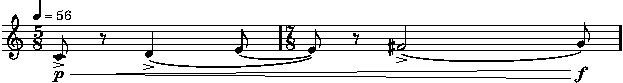
\includegraphics[max width=\textwidth,]{assets/lilypond-a7ec7b445307363d41998bfba7240e5f.pdf}
\end{singlespacing}
\end{abjadbookoutput}

\end{frame}

\begin{frame}[fragile]{Typographic overrides}
\begin{comment}
<abjad>
override(score['Lower Staff']).note_head.style = 'slash'
override(score['Lower Staff']).staff_symbol.line_positions = schemetools.SchemePair(-4, 4)
show(score)
</abjad>
\end{comment}

\begin{abjadbookoutput}
\begin{singlespacing}
\vspace{-0.5\baselineskip}
\begin{minted}{pycon}
>>> override(score['Lower Staff']).note_head.style = 'slash'
>>> override(score['Lower Staff']).staff_symbol.line_positions = schemetools.SchemePair(-4, 4)
>>> show(score)
\end{minted}
\noindent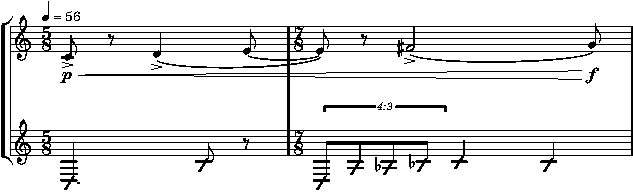
\includegraphics[max width=\textwidth,]{assets/lilypond-4fd5d30f6d67e7dc95e18808899f5ad9.pdf}
\end{singlespacing}
\end{abjadbookoutput}

\end{frame}

\begin{frame}[fragile]{Component Mutation}
\begin{comment}
<abjad>
staff = Staff("c'4 d'4 e'4 f'4 g'4 a'4 b'4 c''4")
show(staff)
shards = mutate(staff.select_leaves()).split([(5, 16)], cyclic=True)
for i, shard in enumerate(shards):
    if i % 2:
        mutate(shard).transpose('+M3')
    attach(Slur(), shard)

show(staff)
</abjad>
\end{comment}

\begin{abjadbookoutput}
\begin{singlespacing}
\vspace{-0.5\baselineskip}
\begin{minted}{pycon}
>>> staff = Staff("c'4 d'4 e'4 f'4 g'4 a'4 b'4 c''4")
>>> show(staff)
\end{minted}
\noindent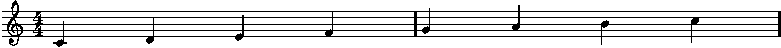
\includegraphics[max width=\textwidth,]{assets/lilypond-2037c19c781fc60f587ffb811c73bee9.pdf}
\begin{minted}{pycon}
>>> shards = mutate(staff.select_leaves()).split([(5, 16)], cyclic=True)
>>> for i, shard in enumerate(shards):
...     if i % 2:
...         mutate(shard).transpose('+M3')
...     attach(Slur(), shard)
...
>>> show(staff)
\end{minted}
\noindent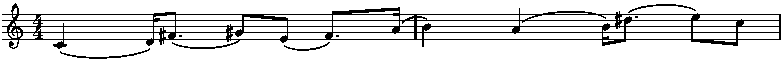
\includegraphics[max width=\textwidth,]{assets/lilypond-d1d1b132557a6e06aabb2a560d1d258e.pdf}
\end{singlespacing}
\end{abjadbookoutput}

\end{frame}

\begin{frame}[fragile]{Object Persistence}
Text
\end{frame}

\begin{frame}[fragile]{Object templating}
Text
\end{frame}
\section{Music}

\begin{frame}{A small concert}
    \begin{description}
        \item[2015] Josiah: \textbf{Invisible Cities (iii): Ersilia} \\
            for chamber orchestra
        \item[2015] Trevor: \textbf{Al-kitab al-khamr} \\
            for eleven players
        \item[2015] Josiah: \textbf{Invisible Cities (ii): Armilla} \\
            for viola duet
        \item[2014] Trevor: \textbf{Krummzeit} \\
            for seven players
    \end{description}
    \begin{center}
        Scores and source code are all available on GitHub.
    \end{center}
\end{frame}

\begin{frame}{Josiah's music}
    \begin{description}
        \item[2015] \textbf{Invisible Cities (iii): Ersilia} \\
            for chamber orchestra
        \item[2015] \textbf{Invisible Cities (ii): Armilla} \\
            for viola duet
        \item[2014] \textbf{Invisible Cities (i): Zaira} \\
            for eight players
        \item[2014] \textbf{Plague Water} \\
            for bari sax, e-guitar, piano and percussion
        \item[2011] \textbf{Aurora} \\
            for string orchestra
        \item[2010] \textbf{Lagartija} \\
            for mixed quartet
    \end{description}
\end{frame}

\begin{frame}{Trevor's music}
    \begin{description}
        \item[2015] \textbf{Al-kitab al-khamr} \\
            for eleven players
        \item[2015] \textbf{Ins Wasser eingeschrieben} \\
            for viola duet
        \item[2014] \textbf{Krummzeit} \\
            for seven players
        \item[2013] \textbf{Traiettorie inargentate} \\
            for cello
        \item[2011] \textbf{L'archipel du corps} \\
            for flute, guitar, accordion \& percussion
        \item[2009] \textbf{Mon seul désir} \\
            for flute, clarinet, violin \& cello
        \item[2008] \textbf{Lidércfény} \\
            for flute, violin \& piano
    \end{description}
\end{frame}

\begin{frame}{Jeff's music}
    \begin{description}
        \item[2015] \textbf{On the Behavior of Climbing Plants} \\
            for chamber orchestra
        \item[2013] \textbf{The World All Around} \\
            for Eb clarinet, prepared piano, and harp
        \item[2013] \textbf{+/-} \\
            for twenty french horns
        \item[2013] \textbf{Enfilade, Moses All, and Future Calendars} \\
            for carillon
        \item[2011] \textbf{Being Pollen} \\
            for solo percussion
    \end{description}
\end{frame}


\section{Integration}

\begin{frame}[fragile]{Integrating with other tools}
    \begin{block}{LaTeX}
        Preprocessing LaTeX input files
    \end{block}
    \begin{block}{Sphinx}
        Extensions for executing Python inline and embedding graphics
    \end{block}
    \begin{block}{IPython}
        Embedding graphics and audio in IPython notebooks
    \end{block}
    \begin{block}{Graphviz}
        Object-oriented toolkit for constructing Graphviz graphs
    \end{block}
\end{frame}
\section{Composition}

\section{Conclusion}

\begin{frame}{Conclusion}
The Abjad API for Formalized Score Control extends the Python programming
language with an open-source, object-oriented model of common-practice music
notation that enables composers to build scores through the aggregation of
elemental notation objects.
\end{frame}

\begin{frame}[fragile]{About the code base}
\begin{markdown}
- 496 public classes
- 387 public functions
- 186,963 lines of code
- 9399 unit tests
- 10190 documentation tests
- 100\% free \& open source
- platform independent
- runs under both Python 2.7, 3.3+ and PyPy
\end{markdown}
\end{frame}

\begin{frame}{Online presence}
    \begin{block}{Documentation}
        http://projectabjad.org
    \end{block}
    \begin{block}{GitHub Repository}
        http://github.com/Abjad/abjad
    \end{block}
    \begin{block}{User Mailing List}
        http://groups.google.com/group/abjad-user
    \end{block}
\end{frame}

\begin{frame}{TENOR 2015 (github.com/Abjad/tenor2015)}
    \begin{figure}
    \begin{centering}
    \begin{tabular}{cc}
    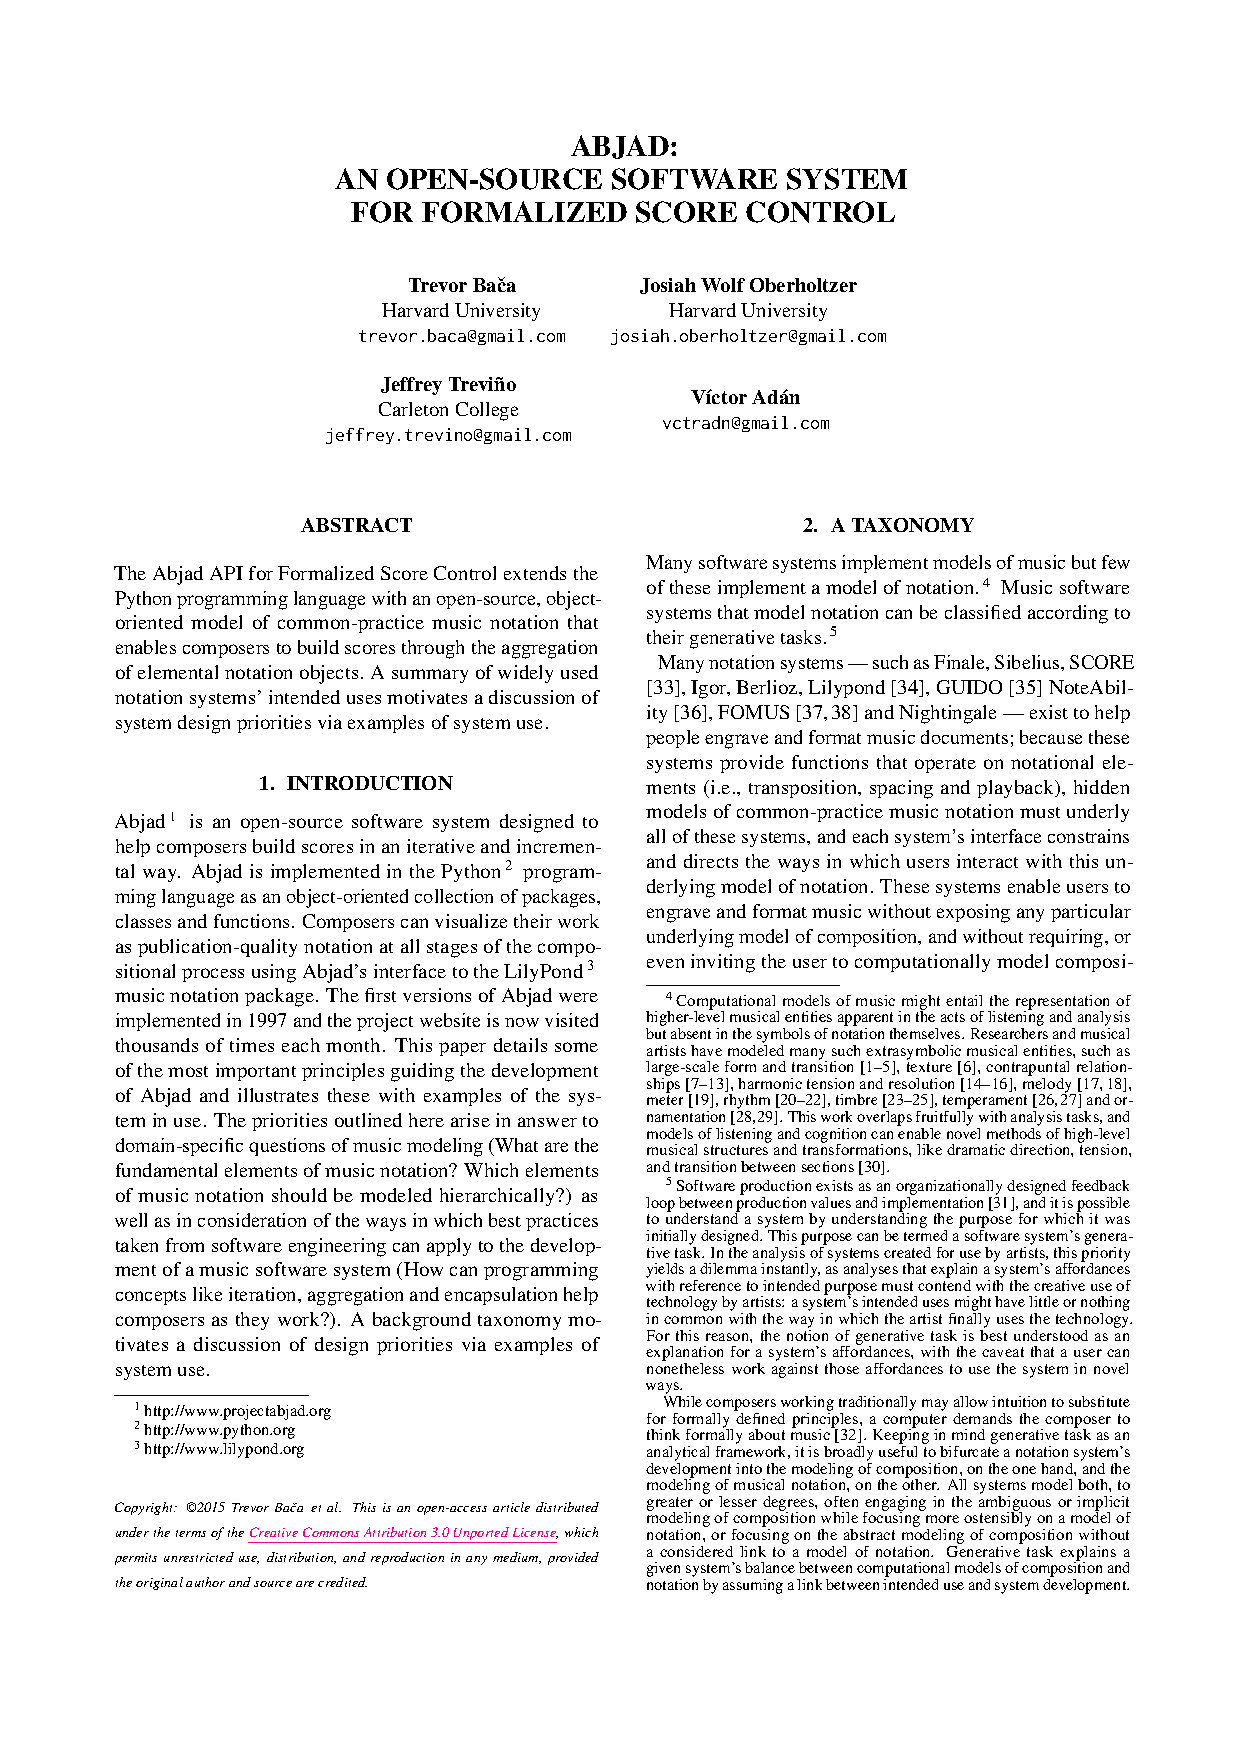
\includegraphics[
        page=1,
        scale=0.2,
        clip=true,
        fbox,
    ]{assets/include-tenor2015.pdf}
    &
    \includegraphics[
        page=2,
        scale=0.2,
        clip=true,
        fbox,
    ]{assets/include-tenor2015.pdf}
    \end{tabular}
    \caption{First International Conference on
        Technologies for Music Notation and Representation,
        May 2015, Paris, France}
    \end{centering}
    \end{figure}
\end{frame}

\begin{frame}{Personal Contacts}
    \begin{columns}[t,onlytextwidth]
        \column{.5\textwidth}
        \textbf{Trevor Ba\v{c}a}
        \begin{itemize}
            \item trevor.baca@gmail.com
            \item trevorbaca.com
            \item github.com/trevorbaca
        \end{itemize}
        \column{.5\textwidth}
        \textbf{Jeffrey Trevi\~{n}o}
        \begin{itemize}
            \item jeffrey.trevino@gmail.com
            \item jeffreytrevino.com
            \item github.com/jefftrevino
        \end{itemize}
    \end{columns}
    \vspace{\baselineskip}
    \textbf{Josiah Wolf Oberholtzer}
    \begin{itemize}
        \item josiah.oberholtzer@gmail.com
        \item josiahwolfoberholtzer.com
        \item github.com/josiah-wolf-oberholtzer
    \end{itemize}
\end{frame}

\end{document}